\subsubsection{\emph{Performance Measures} (PM)}

Avant d'optimiser, nous définissons sur le réseau cyclable des mesures de performance (\emph{Performance Measures}, PM). Cela reprend l'objectif de recherche d'équité, détaillé dans la section \ref{sect:equite}. 

Le procédé est le suivant : nous définissons un PM pour chaque carreau, nous calculons le PM. Ensuite, nous optimisons le réseau cyclable. Enfin, nous mesurons de nouveau le PM sur le réseau cyclable amélioré. Ainsi, nous pouvons comparer l'amélioration du réseau cyclable sur des critères précis.

C'est l'observation de l'existant qui pousse à la création d'un PM, de sorte à le quantifier, et le PM lui même pousse à développer des critères d'optimisation.


% \textcolor{red}{revoir avec derniere partie de ce .tex}

% %---- 

\subsubsection{Critères retenus}


L'objectif est de faire un modèle d'aide à la décision pour la métropole de Tours, afin de trouver les meilleurs tronçons à aménager pour améliorer l'équité du réseau cyclable. Dans notre modélisation, "aménager" un tronçon se traduit par "mettre au minimum son niveau LTS".

Nous avons retenu 3 critères d'optimisation différents :

\begin{enumerate} \label{criteresopti}
    \item le nombre de POI totaux atteints, \label{criterepoi}
    \item la population pouvant atteindre un POI, \label{criterepopu}
    \item le nombre de catégories différentes de POI atteintes par chaque carreau. \label{criterecat}
\end{enumerate}

La problématique de l'optimisation est la suivante : en se donnant une distance maximale entre un noeud délégué et un POI \texttt{dmax}, un niveau LTS maximal pour les tronçons que nous pouvons emprunter et un budget à ne pas dépasser, trouver les meilleurs tronçons à aménager.

\subsubsection{Modèles exacts} \label{modelesexacts}

Une manière d'optimiser le réseau cyclable est d'utiliser la programmation linéaire en nombres entiers (PLNE). 

Pour construire le modèle, nous faisons tout d'abord l'hypothèse suivante : le coût d'une amélioration est proportionnel à la distance de l'arc modifié, le budget peut donc s'exprimer en mètres de route à aménager.

% Les paramètres du modèle sont les suivants :

% Pour représenter le réseau cyclable (c'est à dire toutes les routes et chemins pouvant être empruntés potentiellement par les cyclistes), nous utilisons un graphe orienté $G(X, A)$ avec $X \ ( \vert X \vert = n)$ l'ensemble des nœuds et $A$ l'ensemble des arcs. A chaque arc est associé son coût en distance, et son danger. 



% On dispose également de l'ensemble des carreaux Filosofi couvrant le graphe, appelé $Z$. Nous conservons les carreaux dont la population n'est pas nulle.

% Pour chaque carreau, on trouve le nœud $n_z$ $\in$ $X$ le plus proche du centre. Pour chaque carreau $z$, on dispose d'une liste de POI potentiels, notés $L_z$, représentant les POI potentiellement accessibles depuis $n_z$ en $dmax$ km si l'ensemble du réseau était amélioré, c'est-à-dire si toutes les routes étaient sécurisées. Enfin, la fonction succ($i$) renvoie les successeurs du nœud $i$ dans le graphe $G$, et la fonction pred($i$) renvoie les prédécesseurs du nœud $i$ dans le graphe $G$.


%-----------

Les critères d'optimisation listés en \ref{criteresopti} se traduisent en :

\begin{enumerate}
    \item Minimiser la somme sur tous les carreaux du nombre de POI qui lui sont potentiellement accessibles en moins de \texttt{dmax}, mais qui ne sont pas atteints à cause du danger des voies,
    \item Minimiser la somme sur tous les carreaux du nombre de POI qui lui sont potentiellement accessibles en moins de \texttt{dmax}, mais qui ne sont pas atteints à cause du danger des voies, \textbf{multiplié} par la population de ce carreau,
    \item Maximiser la somme sur tous les carreaux du nombre de catégories de POI atteintes par le carreau parmi celles qui lui sont potentiellement accessibles.
\end{enumerate}

Les POI potentiellement accessibles (PPOI, \emph{Potential POI}) sont les POI qu'il serait possible d'atteindre si le niveau LTS de chaque tronçon de route était assez faible pour que l'on s'autorise à passer dessus, dans la limite de distance \texttt{dmax}. Ils sont toujours potentiellement accessibles par rapport à un carreau, un POI peut être potentiellement accessible pour un carreau mais trop loin pour un autre carreau.Les POI potentiellement accessibles mais non atteints sont donc les POI dans cette catégorie, mais qui se sont pas atteints avec les niveaux LTS réels sur chaque tronçon. 

Nous avons donc les fonctions objectives :

\begin{enumerate} \label{enum:function_obj}
    \item $\Minimize \sum_{z \in \mathcal{Z} } \sum_{p \in \mathcal{L}_z} \overline{PPOI_z^p}$,
    \item $\Minimize \sum_{z \in \mathcal{Z} } \sum_{p \in \mathcal{L}_z} \overline{PPOI_z^p} \times w_z$,
    \item $\Maximize \sum_{z \in \mathcal{Z} } \sum_{c \in \mathcal{C}} cat_c^z$.
\end{enumerate}

Avec :

\begin{itemize}
    \item $Z$ : ensemble des carreaux,
    \item $\mathcal{L}_z$ : visibilité du carreau $z$,
    \item $\overline{PPOI_z^p}=
    \begin{cases}
        1 \text{ si le POI $p$ (potentiellement accessible par $z$) n'est pas atteint,} \\
        0 \text{ sinon,}
    \end{cases}$
    \item $\mathcal{C}$ : ensemble des catégories,
    \item $cat_c^z=
    \begin{cases}
        1 \text{ si la catégorie $c$ est atteinte par le carreau $z$,} \\
        0 \text{ sinon.}
    \end{cases}$
\end{itemize}

On ajoute en plus des variables modélisant les arcs, indiquant si un arc est aménagé ou non, si un arc appartient au chemin entre le carreau $z$ et le POI $p$..., ainsi que des contraintes imposant la distance maximale d'un chemin carreau-POI, le budget à ne pas dépasser, la consistance d'un chemin...

Les modèles complets se trouvent en annexe.

\subsubsection{Heuristiques}\label{sect:heuristiquesopt}

Les heuristiques que j'ai développées sont basées sur l'idée suivante : améliorer les plus courts chemins (PCC) partant d'un carreau et arrivant à un POI accessible par le carreau.

L'hypothèse derrière cela est qu'un bon chemin à améliorer entre un carreau et un POI est souvent le PCC, en particulier pour les POI se trouvant proches d'un carreau.

Pour les heuristiques sur la population et sur le nombre de POI, nous utilisons l'algorithme \ref{hpcc}.  

\begin{algorithm}[H]
\DontPrintSemicolon
\caption{heuristique PCC}
\label{hpcc}
\Donnees{graphe, carreaux, dmax, lts\_max, budget}
\Res{Choix de certains arcs à aménager}
\emph{calculer} les PCC et les stocker dans le vecteur pccs\;
\emph{trier}(pccs) \Comment*[l]{différentes manières de trier le vecteur}\;
\TantQue{pccs non vide}{
    pcc $\leftarrow$ dernier élément de pccs\;
    supprimer le dernier élément de pccs\;
    \PourCh{arc e dans pcc}{
        \Si{budget $\ge$ e.coût \textbf{et} e.amélioré=faux \textbf{et} e.lts $>$ lts\_max}{
            budget $\leftarrow$ budget - e.coût\;
            e.amélioré $\leftarrow$ vrai\;
        }
    }
}
\end{algorithm}

Plusieurs tris sur le vecteur \texttt{pccs} ont été testés : 
\begin{itemize}
    \item trier \texttt{pccs} dans l'ordre décroissant de la distance restante à aménager. Le PCC ayant la distance à aménager la plus courte est donc choisi en premier.
    \item trier \texttt{pccs} dans l'ordre croissant de la population du carreau de départ du PCC. Les PCC partant de la tile ayant le plus d'habitants sont alors choisis en premier.
    \item trier \texttt{pccs} dans l'ordre décroissant du ratio $\fFrac{\text{distance à aménager}}{\text{population du carreau}}$.
\end{itemize}


Une heuristique où l'on s'arrêtait prématurément (voir algo \ref{hpcc2}) a aussi été testée. Comme montré sur les tables \textcolor{red}{mettre}, elle donne des résultats similaires à l'heuristique où tout le budget est dépensé. En revanche, le temps pris par les 2 heuristiques sont aussi similaires (la partie la plus coûteuse étant la construction des PCC). J'ai donc conservé l'heuristique \ref{hpcc}.

\begin{algorithm}[H]
\DontPrintSemicolon
\caption{Heuristique PCC sans utiliser tout le budget}
\label{hpcc2}
\Donnees{graphe, carreaux, dmax, lts\_max, budget}
\Res{Choix de certains arcs à aménager}
\emph{calculer} les PCC et les stocker dans le vecteur pccs\;
\emph{trier}(pccs) 
added\_edges $\leftarrow$ vecteur vide \;
\TantQue{budget $>$ 0 \textbf{et} pccs non vide}{
    pcc $\leftarrow$ dernier élément de pccs\;
    added\_complete\_pcc $\leftarrow$ vrai\;
    \PourCh{arc e dans pcc}{
        \Si{budget $>$ 0}{
            \Si{e.amélioré = faux \textbf{et} e.lts $>$ lts\_max}{
                budget $\leftarrow$ budget - e.coût\;
                e.amélioré $\leftarrow$ vrai\;
                ajouter e à added\_edges\;
            }
        }
        \Comment*[l]{si l'on dépasse le budget, on retire la dernière arête ajoutée}
        \Si{budget $<$ 0}{
            e $\leftarrow$ dernier élément de added\_edges\;
            e.amélioré $\leftarrow$ faux\;
            retirer e de added\_edges\;
            budget $\leftarrow$ budget + e.coût\;
            added\_complete\_pcc $\leftarrow$ faux\;
            \textbf{break}\;
        }
    }
    \Si{added\_complete\_pcc = vrai}{
        supprimer le dernier élément de pccs\;
    }
    \Sinon{
        \textbf{break} \Comment*[l]{on arrête dès qu'on ne peut plus aménager un arc}
    }
}
\end{algorithm}

Pour l'optimisation sur le nombre distinct de catégories atteintes par chaque carreau, nous utilisons l'algorithme \ref{hpccdiv}.

\begin{algorithm}[H]
\DontPrintSemicolon
\caption{heuristique diversité de catégories}
\label{hpccdiv}
\Donnees{Carreaux, dmax, lts\_max, budget}
\Res{Choix de certains arcs à aménager}
\emph{calculer} les PCC et les stocker dans le vecteur pccs\;
pccs $\leftarrow$ pour chaque carreau, pour chaque catégorie, conserver seulement le PCC reliant le carreau au POI de la catégorie auquel il reste le moins à aménager (si le PCC existe) 
\emph{trier\_par\_diversité\_décroissante}(pccs) \Comment*[l]{trier les pcc en fonction du nombre de catégories qu'atteignent leur carreau de départ, dans un objectif d'équité}\;
\TantQue{pccs non vide}{
    pcc $\leftarrow$ dernier élément de pccs\;
    supprimer le dernier élément de pccs\;
    \PourCh{arc e dans pcc}{
        \Si{budget $\ge$ e.coût \textbf{et} e.amélioré=faux \textbf{et} e.lts $>$ lts\_max}{
            budget $\leftarrow$ budget - e.coût\;
            e.amélioré $\leftarrow$ vrai\;
        }
    }
    \Si{le pcc est aménagé entièrement \textbf{et} que sa distance à aménager était non nulle}{
        nombre\_de\_catégories\_atteintes(pcc.carreau)+=1\;
        \emph{trier\_par\_diversité\_décroissante}(pccs)
    }
}
\end{algorithm}

Il faut garder en tête que modifier le nombre de catégories atteintes par un carreau lorsqu'on aménage entièrement un PCC (dont la distance à aménager n'est pas nulle) n'est pas exactement recalculer le nombre de catégories qu'atteingnent tous les carreaux. En effet, une ou plusieurs des arêtes de ce PCC pourraient permettre aussi à un autre carreau d'atteindre une nouvelle catégorie, par effet de bord. Mais cela permet de gagner considérablement en vitesse.

Le calcul des PCC se fait en utilisant le graphe, les carreaux et la distance maximale. Pour chaque carreau, nous appliquons un algorithme de Dijkstra à son noeud délégué et au graphe entier. Pour chaque noeud, nous stockons en plus de son prédecesseur la distance à aménager pour arriver jusqu'à ce noeud (nous stockons la distance à aménager, mais les PCC sont les PCC au sens de la distance totale, et non pas juste la distance à aménager). Voir \ref{algo:dij} \textcolor{red}{faire l'algo ?}.



Cela s'effectue en même temps que le calcul des arcs et noeuds se trouvant dans la visibilité des carreaux, pour économiser du temps de calcul. 

Procéder comme cela nécéssite de DeleteEdgesAndNodesNotInPCC \textcolor{red}{développer}

% \begin{algorithm}[H]
% \label{algo:dij}
% \caption{initialize\_tiles\_visibility\_set\_h(\textit{carreaux}, \textit{dmax}, \textit{lts\_max})}
% \KwOut{Calcul des PCC entre chaque couple la distance à aménager de chaque}

% % initialisation
% \BlankLine
% \CommentSty{// préparation des distances et des piles}
% initialiser tous les nœuds : dist = $\infty$, visité = faux\;
% let \textit{S} $\leftarrow$ pile vide de nœuds\;
% let \textit{R} $\leftarrow$ pile vide pour reset\;
% \textit{u} $\leftarrow$ nœud central de \textit{currTile}\;
% u.dist $\leftarrow 0$, u.distAménager $\leftarrow 0$, u.visité $\leftarrow$ vrai\;
% empiler u dans \textit{S} et \textit{R}\;

% \BlankLine
% \While{\textit{S} non vide}{
%     v $\leftarrow$ dépiler(\textit{S})\;
%     ajouter v à \texttt{currTile.NodeVisibility}\;
%     \For{chaque \textit{e} sortant de v}{
%         w $\leftarrow$ extrémité de \textit{e}\;
%         \tcc{calcul des nouvelles étiquettes}
%         $\delta \leftarrow$ v.dist + e.coût\;
%         $\delta_a \leftarrow$ v.distAménager\;
%         \If{e.LTS > lts\_max}{
%             $\delta_a \leftarrow \delta_a + e.coût$\;
%         }
%         \If{$\delta \le$ dmax \textbf{et} $\delta <$ w.dist}{
%             % mise à jour
%             w.dist $\leftarrow \delta$\;
%             w.distAménager $\leftarrow \delta_a$\;
%             \If{w.visité = faux}{
%                 w.visité $\leftarrow$ vrai\;
%                 empiler w dans \textit{S} et \textit{R}\;
%             }
%             % ajouter l'arête visible
%             ajouter e à \texttt{currTile.EdgeVisibility}\;
%             % stocker prédécesseur et distance à aménager
%             \texttt{currTile.PredAndDist}[\,w.id\,] $\leftarrow$ (v, \(\delta_a\))\;
%         }
%     }
%     % tri de la pile par distance décroissante
%     trier \textit{S} par \texttt{dist} décroissante\;
% }
% \end{algorithm}


\subsubsection{Deux visibilités différentes} \label{sect:2visi}

L'optimisation par CPLEX s'effectue sur deux visibilités différentes : 

\begin{itemize}
    \item La \textbf{visibilité exacte}, où la visibilité d'un carreau comprend tous les arcs qui lui sont à une distance inférieure à la distance maximale \texttt{dmax}. Etant donné que \texttt{dmax} ne peut pas être dépassé lors de la recherche du résultat optimal, ce modèle donne le même résultat que si tout le graphe était visible, la visibilité est bien exacte. Cette technique permet de rendre CPLEX plus rapide, parce qu'on ne créé pas de variables correspondant aux couples carreaux-POI et pour les triplets carreaux-POI-arcs dans un chemin impossibles. Voir figure \ref{fig:exactvisi} \textcolor{red}{mettre ?}.%\par\medskip

    \item La \textbf{visibilité réduite/visibilité PCC}, où la visibilité d'un carreau comprend toutes les arêtes qui sont dans un PCC d'un nœud délégué jusqu'à un point d'intérêt, tout en respectant la contrainte de distance de la visibilité précédente. La visibilité d'un carreau comprend aussi les arêtes se trouvant dans un PCC allant d'un nœud délégué d'un \emph{autre} carreau à un POI, tant que ces arêtes sont à moins de \texttt{dmax} de distance du carreau. Voir figure \ref{fig:smallvisi}.
\end{itemize} 

\begin{figure}[H]
    \centering
    \begin{subfigure}[t]{0.3\textwidth}
        \centering
        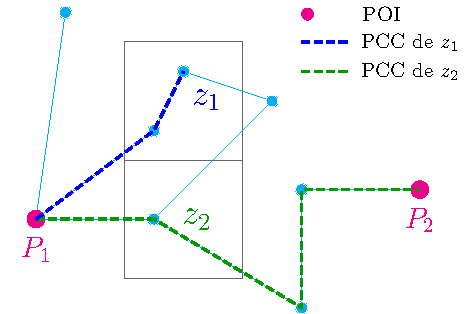
\includegraphics[width=0.92\linewidth]{PDFs/graph.pdf}
    \caption{Considérons un graphe avec 2 POI. Supposons que, en une distance \texttt{dmax}, $P_1$ soit accessible à la fois par $z_1$ et $z_2$, un PCC existe donc de $z_1$ à $P_1$ et de $z_2$ à $P_1$. Supposons aussi que $P_2$ ne soit accessible que par $z_2$. Un PCC existe de $z_2$ à $P_2$, mais pas de $z_1$ à $P_2$. }
    \end{subfigure}
    \hfill
    \begin{subfigure}[t]{0.3\textwidth}
        \centering
        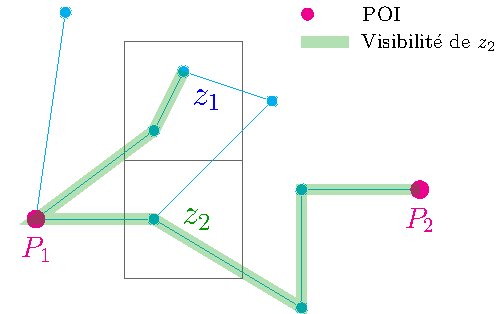
\includegraphics[width=1\linewidth]{PDFs/visi_z2.pdf}
    \caption{Si l'on suppose qu'en passant seulement par un arc hachuré en vert ou bleu, en moins de \texttt{dmax} il est possible d'aller de $z_2$ jusqu'à $z_1$, la visibilité de $z_2$ est celle ci dessus.}
    \end{subfigure}
    \hfill
    \begin{subfigure}[t]{0.3\textwidth}
        \centering
        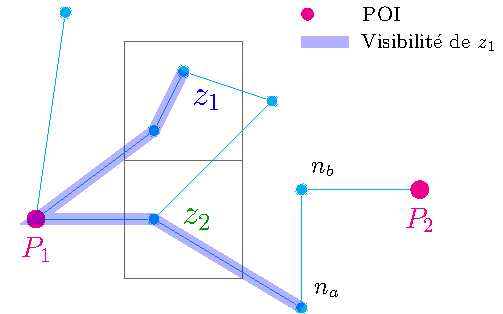
\includegraphics[width=1\linewidth]{PDFs/visi_z1.pdf}
    \caption{Si l'on suppose qu'en passant seulement par un arc hachuré en vert ou bleu, en moins de \texttt{dmax} il est possible d'aller de $z_1$ jusqu'à $n_a$, mais pas jusqu'à $n_b$, la visibilité de $z_1$ est celle ci dessus.}
    \end{subfigure}
    \caption{Visibilité réduite}
    \label{fig:smallvisi}
\end{figure}

Les noeuds visibles sont ceux qui appartiennent à un arc dans la visibilité.

La visibilité pour les heuristiques est toujours la seconde. L'intérêt de faire un modèle exact sur la seconde visibilité est d'avoir un modèle plus rapide que le modèle exact sur la visibilité exacte, et aussi de pouvoir comparer les performances des heuristiques.

La valeur objective dépend aussi de la visibilité sur laquelle on la calcule.



\subsubsection{Pertinence des résultats trouvés}

Les modèles utilisés sont incomplets par rapport à la réalité du terrain. Ils ne se soucient pas, par exemple, d'à quel point il est facile d'aménager tel ou tel tronçon. 

L'hypothèse sur le budget est simpliste. En réalité, le budget alloué à l'aménagement des tronçons peut varier en fonction de nombreux facteurs, tels que la complexité des travaux, les contraintes techniques, ou encore les enjeux environnementaux.

Les modèles ne prennent pas non plus en compte les effets à long terme des aménagements proposés. Par conséquent, les résultats obtenus doivent être interprétés avec prudence et complétés par des études de terrain et des consultations avec les acteurs locaux.

C'est l'intérêt de travailler avec des cartographes, qui connaissent la réalité du terrain et ces problématiques.